\redheader
\begin{frame}{2C: Tolkning av integralet}
Arealet av området mellom en graf og førsteaksen har samme enhet som produktet av enhetene på aksene
    \begin{figure}
        \centering
        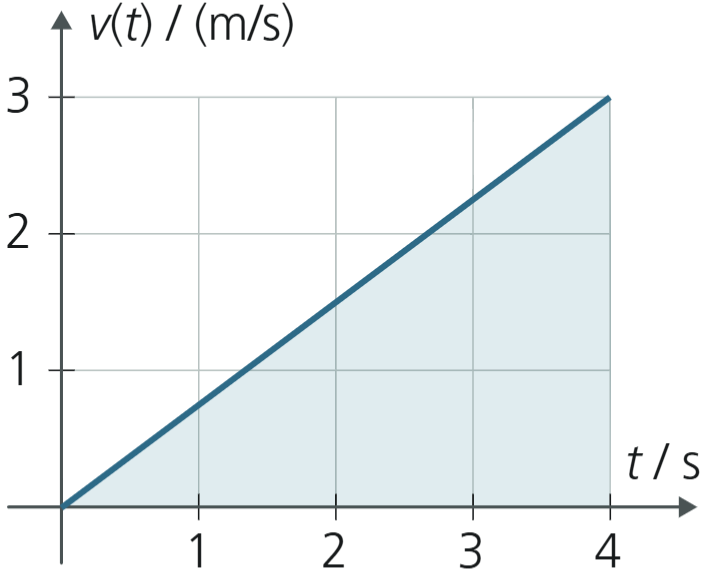
\includegraphics[width=0.5\linewidth]{R2-K2C-1.png}
    \end{figure}
\end{frame}

\greenheader
\begin{frame}{2C: Eksempel 7 side 114}
Modellen beskriver hvor mange liter vann som renner ut av et akvarium per sekund.
\begin{equation*}
    V(t)=3,8\cdot e^{-0.05t} 
\end{equation*}
Arealet under grafen har enheten liter.\\

Hvor mye vann renner ut i løpet av det første minuttet? 
\begin{figure}
    \centering
    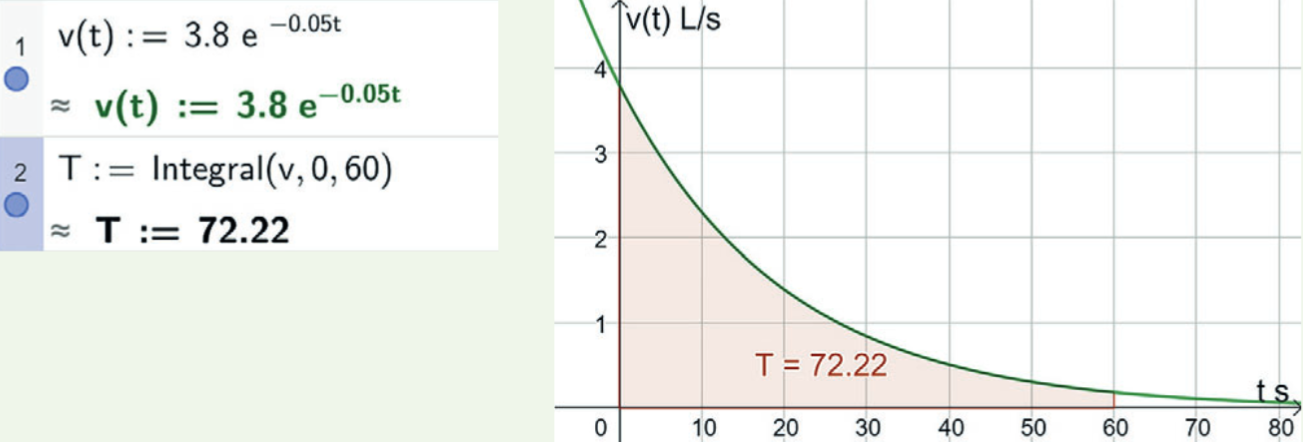
\includegraphics[width=0.8\linewidth]{R2-K2C-2.png}
\end{figure}
\end{frame}

\redheader
\begin{frame}{2C: Arealet under førsteaksen}
    La $A$ være arealet av området avgrenset av grafen til den kontinuerlige funksjonen $f$, x-aksen og linjene $x=a$ og $x=b$.\\
    \begin{align*} 
    \text{Arealet }  A&=\int_a^bf(x)\;dx \text{   hvis området ligger over x-aksen.}\\
       \text{Arealet }  A&=-\int_a^bf(x)\;dx \text{   hvis området ligger under x-aksen.}
       \end{align*}
       
    \medskip
    Hvis området ligger delvis over og delvis under x-aksen, må vi dele det opp i flere deler og summere delarealene.
\end{frame}


\greenheader\begin{frame}{2C: Eksempel 8 side 117}
\begin{figure}
    \centering
    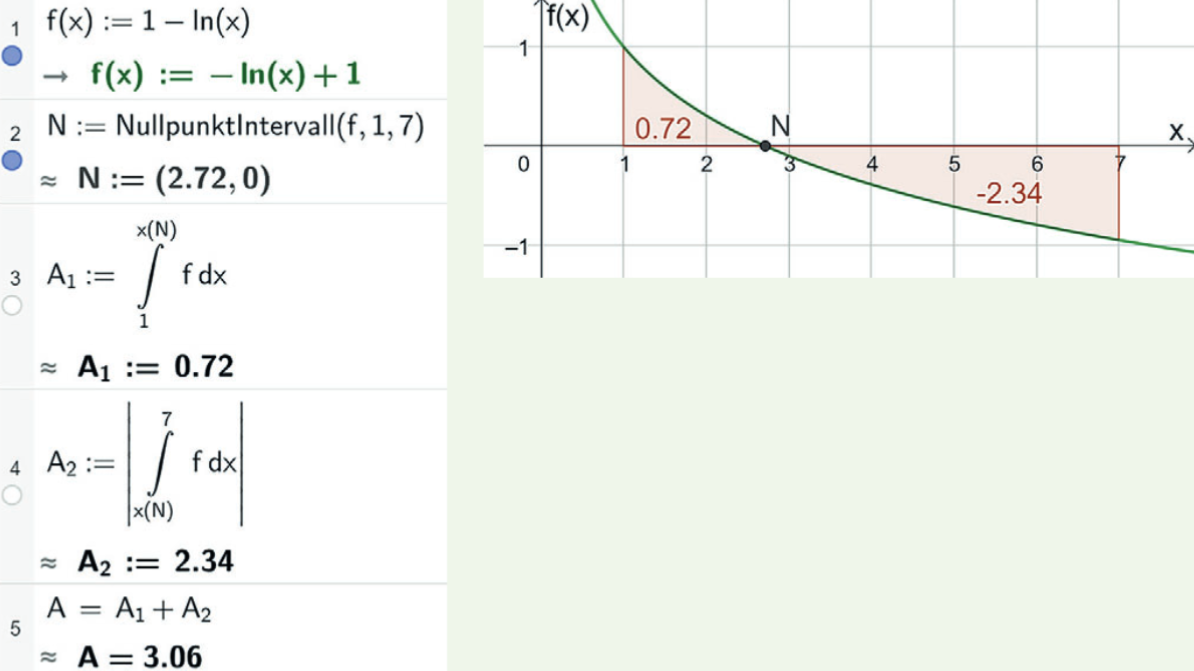
\includegraphics[width=0.9\linewidth]{R2-K2C-3.png}
\end{figure}
\end{frame}

\greenheader\begin{frame}{2C: Eksempel 10 side 122}
\begin{figure}
    \centering
    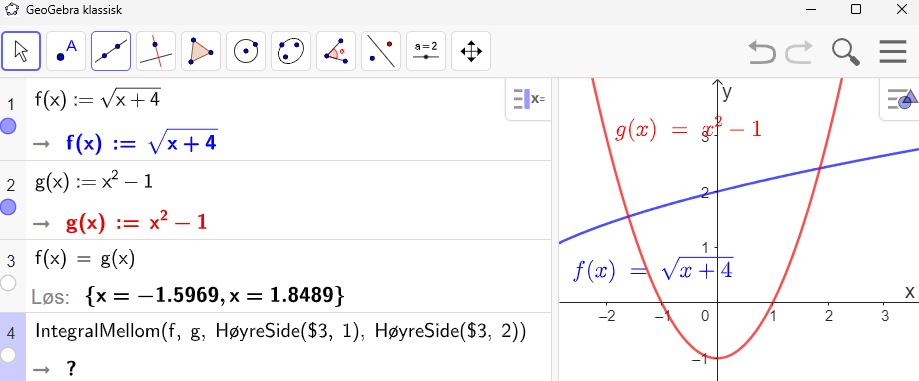
\includegraphics[width=\linewidth]{R2-K2C-4.png}
\end{figure}
\end{frame}

\greenheader\begin{frame}{2C: Eksempel 10 side 122}
\begin{figure}
    \centering
    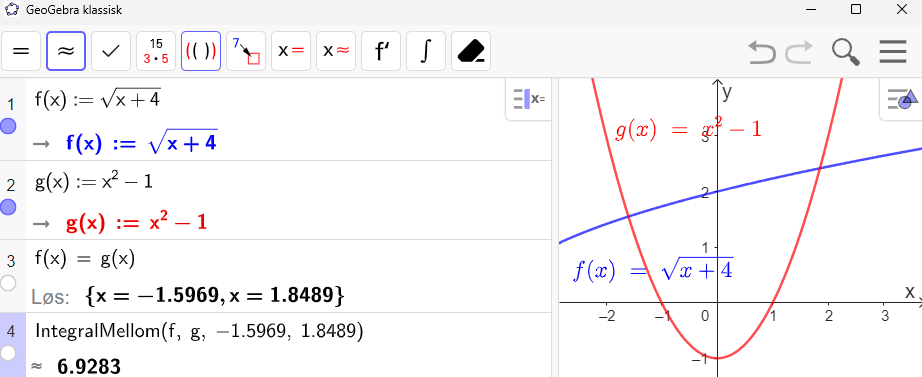
\includegraphics[width=\linewidth]{R2-K2C-5.png}
\end{figure}
\end{frame}

\redheader
\begin{frame}{2C: Arealet mellom to grafer}
    \begin{columns}
        \begin{column}{0.3\linewidth}
            \begin{figure}
                \centering
                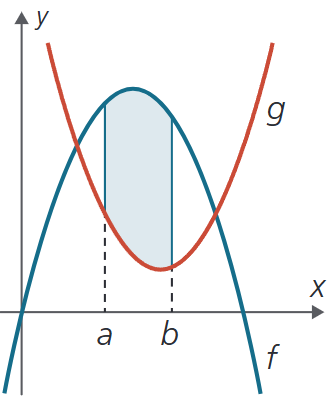
\includegraphics[width=\linewidth]{R2-K2B-12.png}
            \end{figure}
        \end{column}
        \begin{column}{0.6\linewidth}
            Hvis \(f(x)\geq g(x)\) for alle \(x\) i \([a,b]\), er arealet av området mellom grafene til \(f\) og \(g\), og linjene \(x=a\) og \(x=b\) gitt ved
            \begin{equation*}
                A = \int_a^b (f(x) - g(x)) \;dx
            \end{equation*}
        \end{column}
    \end{columns}
\end{frame}

\greenheader\begin{frame}{2C: Eksempel 10 side 122}
\begin{figure}
    \centering
    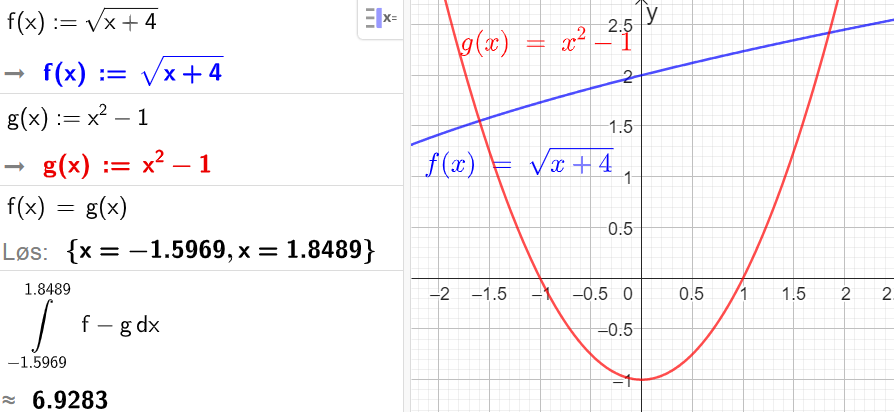
\includegraphics[width=\linewidth]{R2-K2C-7.png}
\end{figure}
\end{frame}

\greenheader
\begin{frame}[fragile]{2C: Areal mellom funksjonene f og g i python (hvis dere vil)}
\begin{minted}[fontsize=\footnotesize]{python}
from pylab import *

def f(x):
  return (x+4)**0.5      # f(x) = kvadratroten av (x+4)

def g(x):
  return x**2 - 1        # g(x) = x^2 - 1

# Skjæringspunktene mellom f og g (løst på forhånd)
a = -1.5969  # Nedre grense
b =  1.8489  # Øvre grense

# Lager en liste med 100 jevnt fordelte x-verdier mellom a og b
x = linspace(a, b, 100)

# Arealet mellom f og g finner vi ved å integrere (f(x) - g(x))
# Her bruker vi trapesmetoden (numerisk tilnærming)
svar = trapezoid(f(x) - g(x), x)
print(svar) # Oputput: 6.927568467295032
\end{minted}
\end{frame}


\redheader
\begin{frame}{2C: Gjennomsnittsverdiern til en funksjon i intervallet $[a, b]$}
Gjennomsnittsverdien til en kontinuerlig funksjon \(f\) i intervallet \([a,b]\) er gitt ved
\[\text{Gjennomsnittsverdi} = \frac{1}{b-a}\int_a^b f(x) \; dx.\]
\begin{figure}
    \centering
    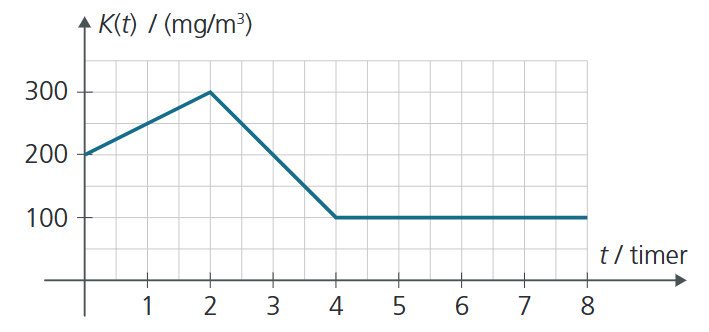
\includegraphics[width=0.6\linewidth]{R2-K2B-13.png}
\end{figure}    
\end{frame}

\greenheader
\begin{frame}{2C: Oppgave 2.51 side 126}
    På en fabrikk der det skilles ut et skadelig stoff, ble konsentrasjonen av stoffet målt gjennom en hel arbeidsdag.\(K(t)\) er konsentrasjonen ved tidspunktet \(t\). Arbeidsmiljøloven krever at den gjennomsnittlige konsentrasjonen i løpet av arbeidsdagen ikke overstiger \(140\,\mathrm{mg}/\mathrm{m}^3\). Var kravet i arbeidsmiljøloven oppfylt denne dagen?

\begin{figure}
    \centering
    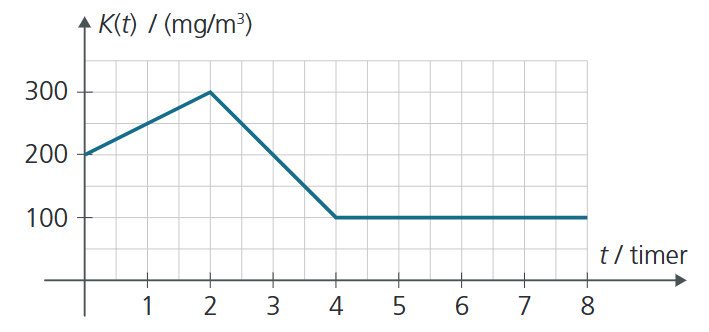
\includegraphics[width=0.6\linewidth]{R2-K2B-13.png}
\end{figure}
\end{frame}

\magentaheader
\begin{frame}{2C: Buelengde til en graf i \([a, b]\) (Utforsk side 126)}
Lengden av grafen til \(f\) i intervallet \([a, b]\) kan tilnærmes ved å summere små linjestykker:
\[
s_i \approx \sqrt{(\Delta x)^2 + (f(x_{i+1}) - f(x_i))^2}
\]
Den eksakte buelengden er gitt ved
\[
s = \int_a^b \sqrt{1 + (f'(x))^2} \; dx
\]

    \begin{figure}
        \centering
        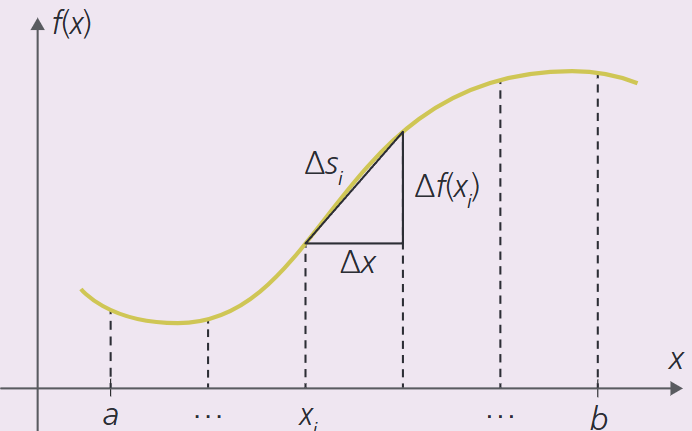
\includegraphics[width=0.4\linewidth]{R2-K2C-8.png}
    \end{figure}
\end{frame}



